\documentclass{article}
\usepackage{amsmath}
\usepackage{hyperref}
\usepackage{float}
\usepackage{graphicx}
\usepackage{caption}

\author{Erin Angelini}
\title{Documentation for mean-field model (Matlab)}
\begin{document}
\maketitle

\section{Overview of functions}
The following Matlab functions constitute the mean-field model of mitotic spindle rotation in \emph{C. elegans} embryos. \\[3pt]

\noindent\texttt{Main.m}: This is the function that implements the full model. That is, it calculates the potential energy $W(\alpha)$ at angles $\alpha$ from 0 and $\pi$. See \S\ref{params} for more information about the step size of $\alpha$. This function takes inputs on both the cell geometry (\texttt{a} and \texttt{b}) and the setup of the spindle (\texttt{ctr}, \texttt{phi\_1}, \texttt{phi\_2}, \texttt{push}, \texttt{AP}, \texttt{LD}, \texttt{elas}; see \S\ref{params}). The output of \texttt{Main.m} is the energy landscape \texttt{W} over the range of angles \texttt{A} $=[0,\pi]$ in vector form. It also plots \texttt{W} against \texttt{A}. 
\\[3pt]

\noindent\texttt{MainWithFilter.m}: This function is the exact same as \texttt{Main.m}, except that it puts the output \texttt{W} through a high-pass filter (to clean up the curve) before plotting. Note that this file is \textbf{only useful for the symmetric well case}: the high-pass filter loses all information about asymmetry in the wells.
\\[3pt]

\noindent\texttt{parameters.m}: This script contains all the fixed parameters in the model (see \S\ref{params}). It is called by \texttt{Main.m} at the beginning of the file; it is also called by \texttt{work.m}, \texttt{torque.m}, and \texttt{find\_prob.m}. It does not take any inputs and its output is to load the fixed parameters onto the workspace.
\\[3pt]

\noindent\texttt{alpha\_halfplane.m}: This function is called by \texttt{Main.m} before calculating \texttt{W}. Its inputs are \texttt{a}, \texttt{r\_N}, \texttt{ctr}, \texttt{phi\_1}, and \texttt{phi\_2} (\S\ref{params}). The purpose of this function is to calculate the angles at which the leading and lagging ends of each MT aster are above or below the $x$-axis (for ease of future calculations in \texttt{torque.m}). It saves these angles to two .mat files, \texttt{halfplane1.mat} and \texttt{halfplane2.mat}, which are later loaded by \texttt{torque.m}.
\\[3pt]

\noindent\texttt{equal\_arcsCircle.m}: This function is called by \texttt{Main.m} in the case that the cell is perfectly circular (i.e. aspect ratio = 1 or \texttt{a} = \texttt{b}). It calculates the locations of the cortical dyneins in terms of the parameter $t$ that parameterizes the boundary of the cell. The output of this function is a vector of these positions.
\\[3pt]

\noindent\texttt{equal\_arcsHannah.m}: This function is called by \texttt{Main.m} in the case that the cell is perfectly circular (i.e. aspect ratio $\ne$ 1 or \texttt{a} $\ne$ \texttt{b}). It calculates the locations of the cortical dyneins in terms of the parameter $t$ that parameterizes the boundary of the cell. The output of this function is a vector of these positions.
\\[3pt]

\noindent\texttt{let99.m}: This function calculates the beginning and end positions of the Let-99 push band in the case that the band is present (i.e. \texttt{push = `on'}, see \S\ref{params}). Again, these positions are in terms of the parameter $t$ that parameterizes the boundary of the cell. Given the cell resolution (\texttt{a} and \texttt{b}) and a fixed arc-length \texttt{arc}, it outputs a vector \texttt{tvec} that contains the beginning and end positions of the push band. In the case that there is no push band present (i.e. \texttt{push = `off'}, see \S\ref{params}), \texttt{tvec} is an empty vector.
\\[3pt]

\noindent\texttt{work.m}: This is the function called by \texttt{Main.m} that actually calculates the energy landscape. It has the same inputs as \texttt{Main.m} plus an additional input \texttt{alpha}, which is the current angular orientation of the spindle. It calculates the potential energy of the spindle at \texttt{alpha} by approximating the integral of the torque function from angle 0 to angle \texttt{alpha}. This integral is approximated numerically by a Riemann sum of step size \texttt{d\_alpha} (see \S\ref{params}) that calls \texttt{torque.m}.
\\[3pt]

\noindent\texttt{torque.m}: This function, which has all the same inputs as \texttt{work.m}, calculates the total torque on the spindle at a given angular orientation \texttt{alpha}; this value is its output. The following seven functions (\texttt{find\_env\_pi.m} to \texttt{find\_pull.m}) are the helper functions that allow it to do so. 
\\[3pt]

\noindent\texttt{find\_env\_pi.m}: This function finds the beginning and end positions of the MT aster along the cell boundary (in terms of the boundary parameter $t$) given that the aster's angular spread \texttt{phi\_i} is equal to $\pi$. Its inputs are $\texttt{a},$ $\texttt{b}$, \texttt{r\_N}, and \texttt{ctr}, and its output are the beginning and end points of the aster. It finds these points by selecting the correct roots from symbolic solutions for the intersection of the line defined by the aster spread and the cell boundary (Figure \ref{envPi}). This function is called separately for each of the upper and lower (or ``mother'' and ``daughter'') asters. 
%\\[3pt]

\begin{figure}[H]
\centering
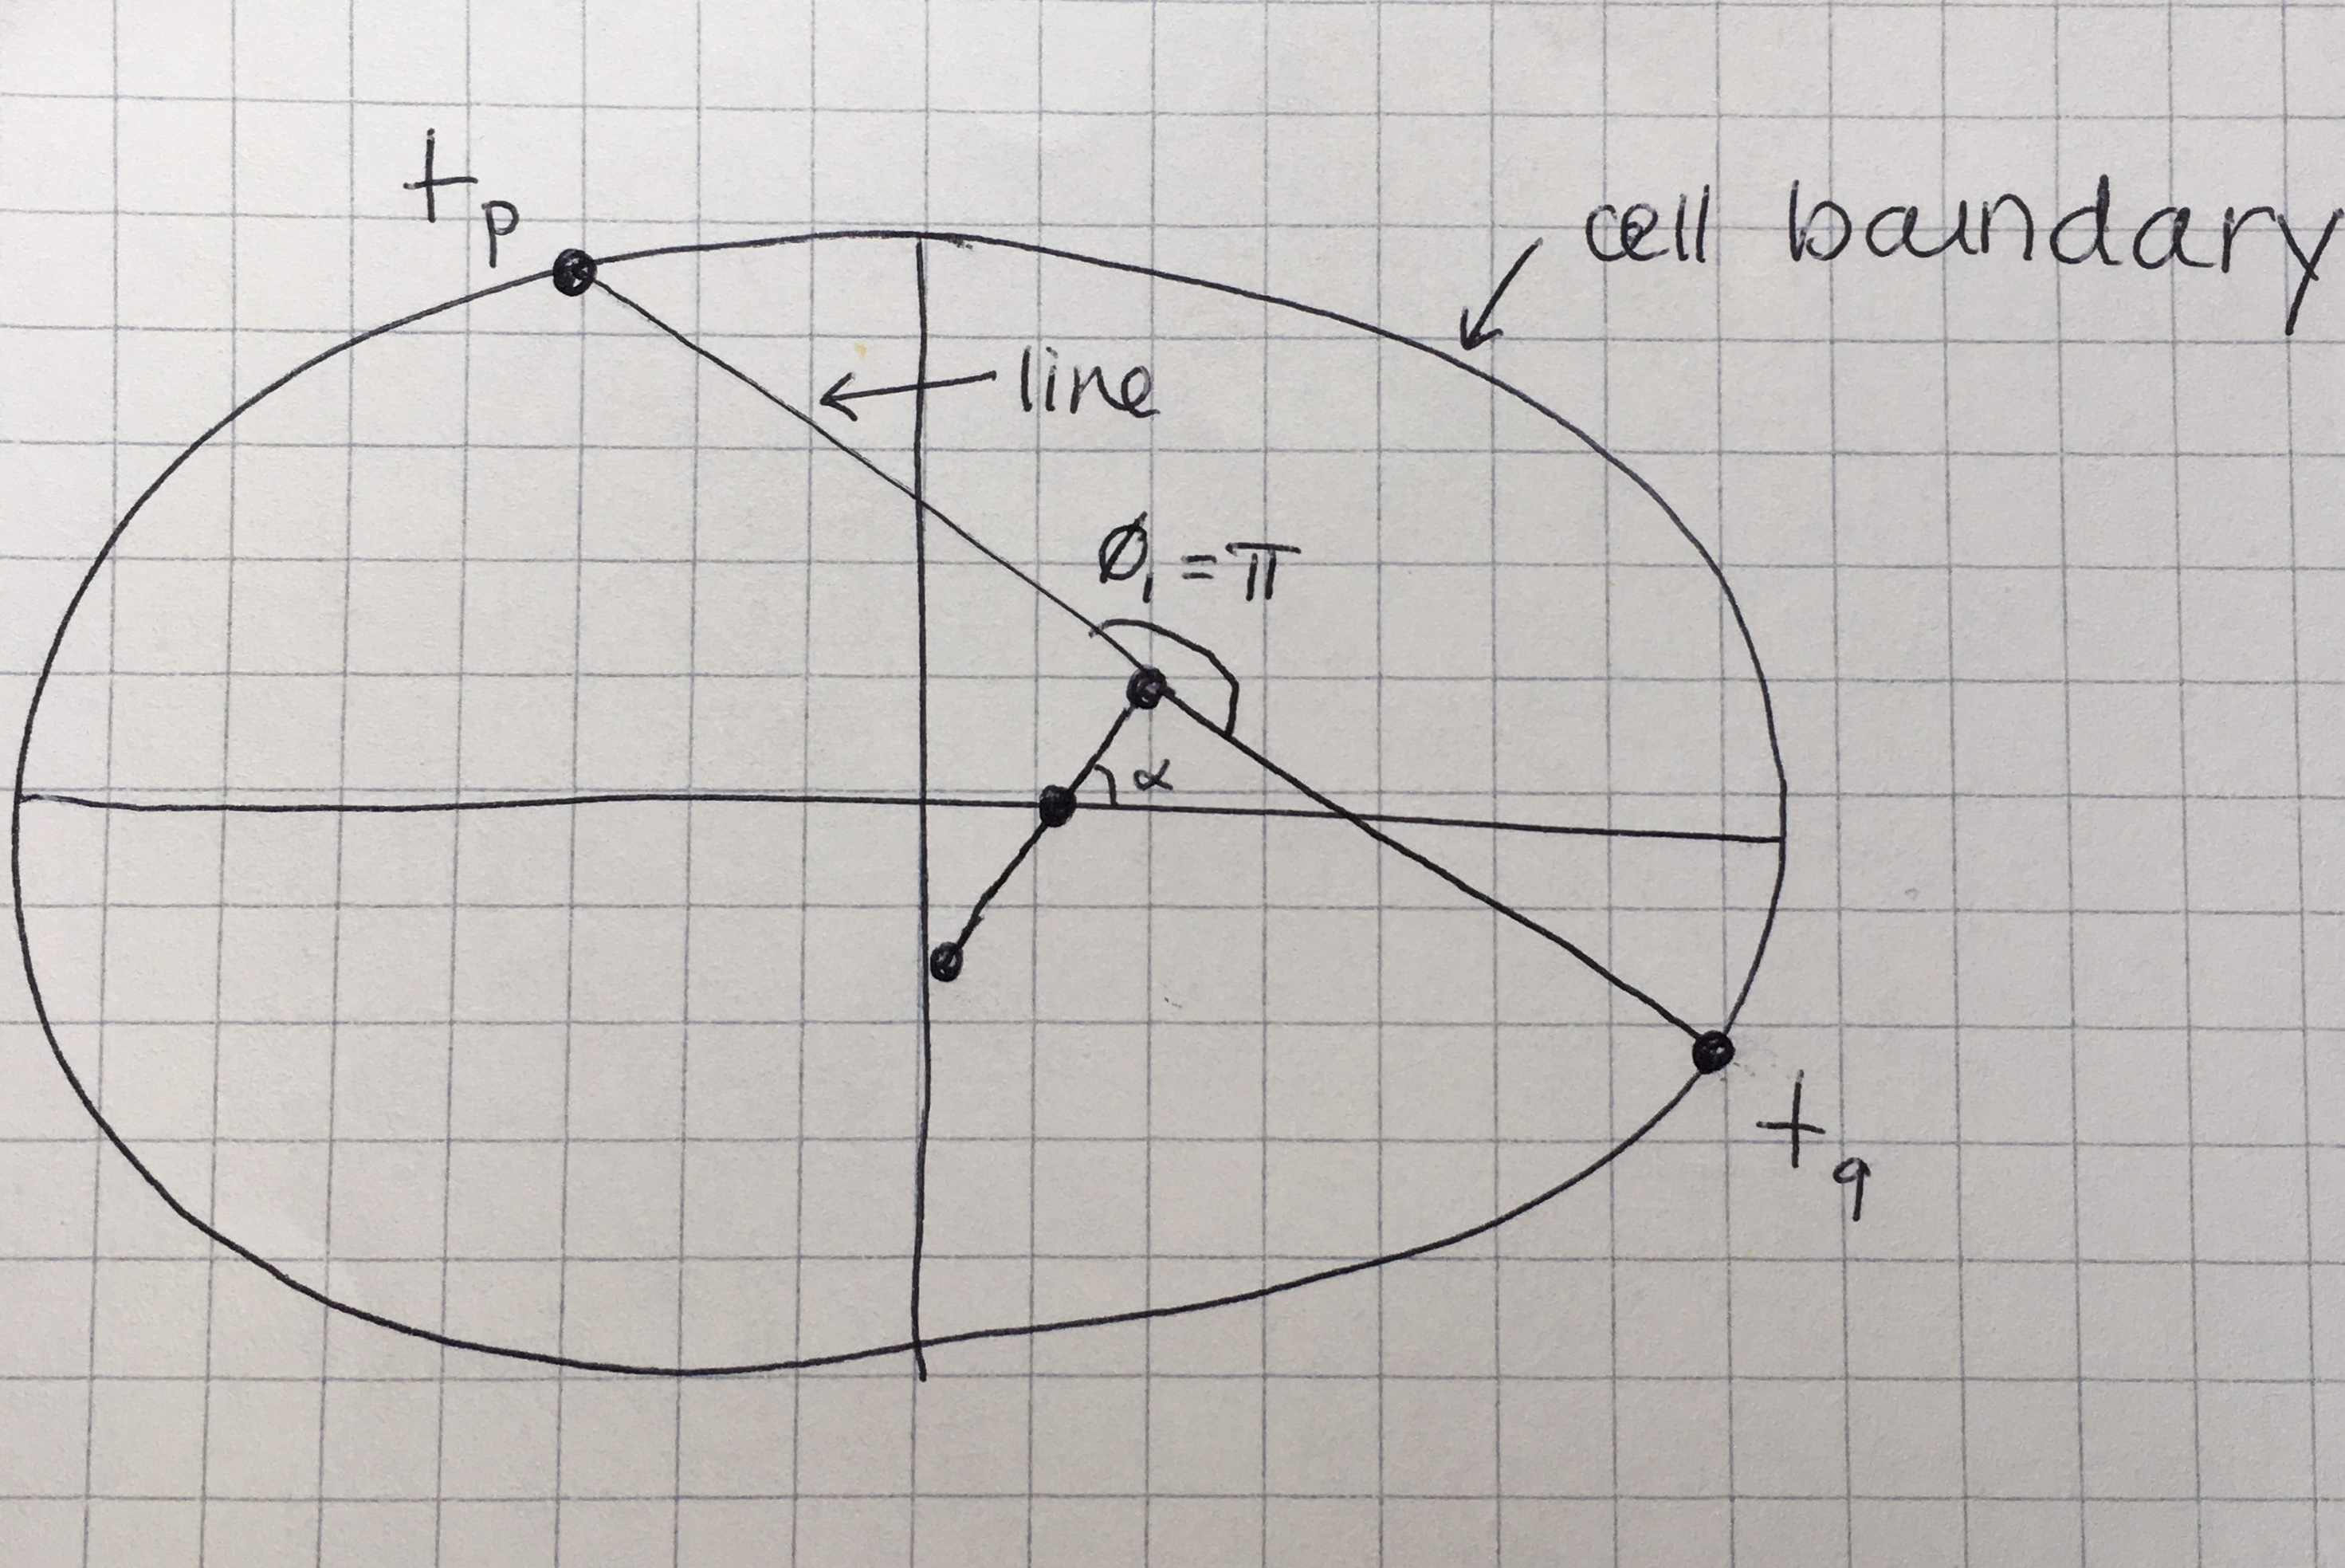
\includegraphics[width=0.75\textwidth]{figures/envPi.jpg}
\caption{Geometric setup for the function \texttt{find\_env\_pi.m}.}
\label{envPi}
\end{figure}

\noindent\texttt{find\_env\_notpi.m}:  This function finds the beginning and end positions of the MT aster along the cell boundary (in terms of the boundary parameter $t$) given that the aster's angular spread \texttt{phi\_i} is less than $\pi$. It takes the same inputs as \texttt{find\_env\_pi.m} plus the aster spread \texttt{phi\_i}. It also takes the angles from \texttt{alpha\_hlafplane} as inputs. It makes calls to \texttt{find\_env\_pi.m} and \texttt{find\_end.m}, and uses the following geometric setup to compute the beginning and end of the MT aster with correct spread \texttt{phi\_i} (Figure \ref{envNotPi}). This function is also called separately for each of the upper and lower (or ``mother'' and ``daughter'') asters. 
\\[3pt]

\begin{figure}[H]
\centering
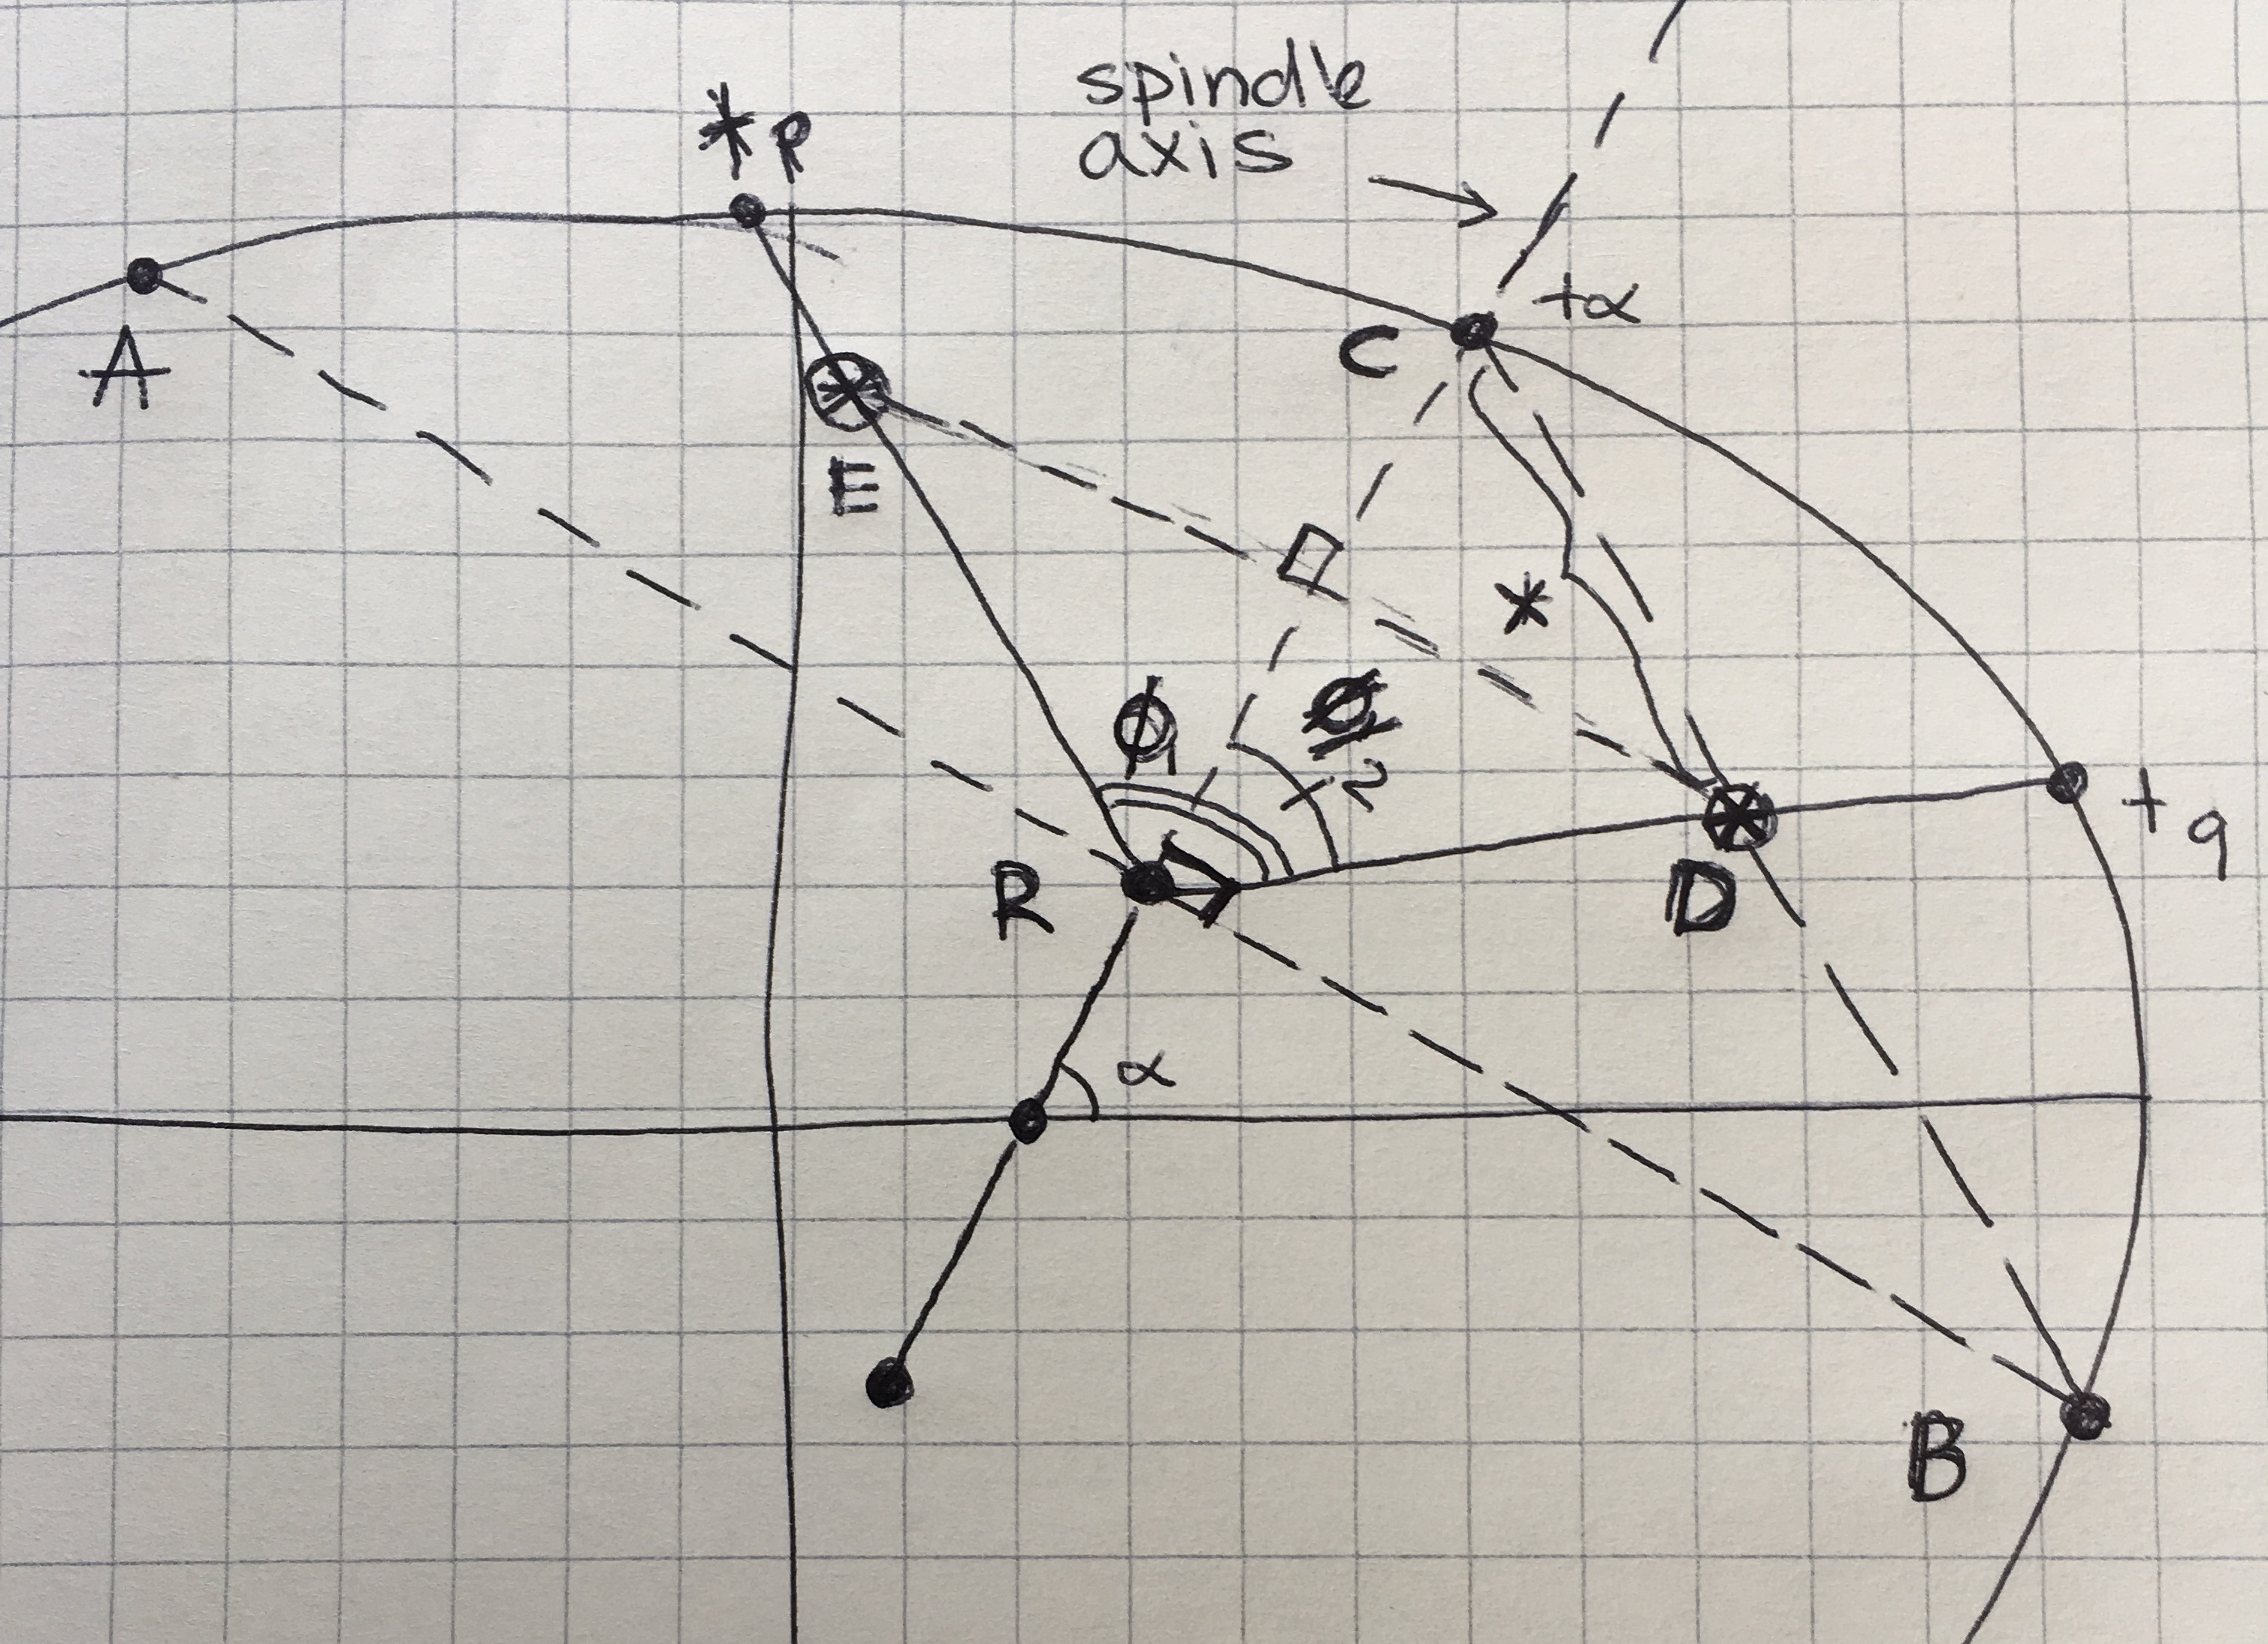
\includegraphics[width=0.75\textwidth]{figures/envNotPi.jpg}
\caption{Geometric setup for the function \texttt{find\_env\_notpi.m}.}
\label{envNotPi}
\end{figure}

\noindent\texttt{find\_end.m}: This function finds the point \texttt{D} in the above configuration (Figure \ref{envNotPi}). It does so by finding the line segment with length \texttt{x} (found by the law of sines as we know $|$\texttt{CR}$|$, $|$\texttt{CB}$|$, $\angle$\texttt{RCD}, and $\angle$\texttt{DCR} = \texttt{phi\_i/2}) in the direction of the line segment \texttt{CB} (Figure \ref{envNotPi}). Call this segment \texttt{CD} (Figure \ref{envNotPi}). Using geometric properties of vector addition, we obtain the point (i.e. vector) \texttt{D} by adding the vector \texttt{C} to the vector \texttt{CD} (Figure \ref{envNotPi}). This point \texttt{D} is crucial for finding the lagging endpoint of the MT aster because it allows the function \texttt{find\_env\_notpi.m} to define a line from the MTOC (point \texttt{R}) to the cell boundary that makes angle \texttt{phi\_i/2} with the spindle axis (Figure \ref{envNotPi}). The function \texttt{find\_env\_notpi.m} then reflects \texttt{D} across the spindle axis to the point \texttt{E}, and similarly finds the leading endpoint of the aster (Figure \ref{envNotPi}).
\\[3pt]

\noindent\texttt{find\_dyneins.m}: Given the endpoints \texttt{t\_p} and \texttt{t\_q} of the MT aster (along with the vector of all dynein positions \texttt{set\_psi} and some other inputs), this function finds the dynein positions that are within the MT aster. It stores these dyneins in the output vector \texttt{env\_d} It also takes the Let-99 band positions \texttt{tvec}, and places the dynein positions in the Let-99 band that overlap with the aster in a separate vector \texttt{let} (so these positions are NOT included in \texttt{env\_d}). This output vector now contains the positions along the boundary in the Let-99 band where MTs will grow up against the boundary (i.e. no dyneins) and create pushing forces.
\\[3pt]

\noindent\texttt{find\_sintheta.m}: This function finds the sine of the angle \texttt{theta\_i} made by each MT in the aster and the spindle axis. We need the sines of these angles in order to calculate the torque on the spindle center (i.e. the pronucleus). This function is called separately for each MT aster, as well as for the MTs making contact with dyneins (\texttt{env\_d}) versus those in the push band (\texttt{let}). This function also implements MT sliding and elasticity. If this feature is present (i.e. \texttt{elas = `on'}), then this function perturbs each angle \texttt{theta\_i} with a random angle \texttt{omega} (uniformly sampled from the angle between the two adjacent dynein locations) before calculating the sines.
\\[3pt]

\noindent\texttt{find\_prob.m}: This function is for implementing the anterior-to-posterior difference in MT-dynein binding probabilities (which itself is for scaling down the anterior forces). If this difference is present (i.e. \texttt{AP = `on'}), it loops through the vector of dynein positions \texttt{env\_d} and builds a vector \texttt{myProbs} of corresponding binding probabilities depending on if the dynein is in the anterior region or the posterior region. The anterior-to-posterior split is defined at the 60:40 egg-length mark (\texttt{0.2*a}), and should be kept as such unless we get new experimental findings. Similarly, we want to fix the posterior and anterior binding probabilities (\texttt{P\_p} and \texttt{P\_a}, respectively) fixed, as these are taken from the original study by Coffman \emph{et al}. Otherwise, if there is no anterior-to-posterior difference in place (i.e. \texttt{AP = `off'}), then the vector of probabilities contains all ones. This function is called separately for each MT aster.
\\[3pt]

\noindent\texttt{find\_pull.m}: This function is for implementing length dependent pulling forces. If length dependence is in place (i.e. \texttt{LD = `on'}), then it loops through the vector of dynein positions \texttt{env\_d} and builds a vector \texttt{myForces} of corresponding pulling forces. If not (i.e. \texttt{LD = `off'}), then the vector of pulling forces contains all ones (i.e. pulling force is constant and equal to 1).
\\[3pt]

\noindent\texttt{ellipse.m}: This function is not used in calculating the energy landscape, but is used for plotting purposes. Specifically, it plots the boundary of the cell given the dimensions \texttt{a} and \texttt{b}. There is a commented out section of code in \texttt{torque.m} that calls this function as part of a plot of the complete spindle setup (dynein locations, MT asters, etc.). This function is called separately for each MT aster.
\\[3pt]

\noindent\texttt{PDFplotCTRL.m}: Given the ellipse major axis \texttt{a}, this function plots the steady state p.d.f. $p(\alpha)$ corresponding to $W(\alpha)$, for the case that \texttt{b = 15} and the asters are symmetric (control case, i.e. no \texttt{push} no \texttt{AP}, no \texttt{LD}, no \texttt{elas}). It does so by loading the .mat file of scale factors (\texttt{k = k\_1*Wmax}, where \texttt{Wmax} is the maximum value of \texttt{W}, and \texttt{k\_1} is a pre-fit parameter; see \S\ref{fit}) and plotting the function $p(\alpha) = Ne^{-\texttt{k}W(\alpha)}$ ($N$ is a normalization constant).

\subsection{Inputs \& parameters}
\label{params}

\begin{description}
\item[\texttt{a}:] Ellipse/cell major axis (i.e. half-length of $x$-axis, values between 15-30)
\item[\texttt{b}:] Ellipse/cell minor axis (i.e. half-length of $y$-axis, values between 15-25)
\item[\texttt{ctr}:] Spindle-center position $x$-coordinate
\item[\texttt{phi\_1}:] Upper MT aster spread, between 0 and $\pi$
\item[\texttt{phi\_2}:] Lower MT aster spread, between 0 and $\pi$
\item[\texttt{push}:] String (\texttt{`on'} or \texttt{`off'}), for push band
\item[\texttt{AP}:] String (\texttt{`on'} or \texttt{`off'}), for anterior-to-posterior difference
\item[\texttt{LD}:] String (\texttt{`on'} or \texttt{`off'}), for length-dependent pulling forces
\item[\texttt{elas}:] String (\texttt{`on'} or \texttt{`off'}), for MT slipping and elasticity
\item[\texttt{r\_N}:] Nuclear/spindle radius
\item[\texttt{b\_basal}:] Set equal to 15 (wild type = 15, where \texttt{a} = 25)
\item[\texttt{a\_basal}:] Set equal to 15 (for wild type when elongating $y$-axis)
\item[\texttt{a\_WTscale}:] Wild type dimension (= 40) for scaling up volume
\item[\texttt{b\_WTscale}:] Wild type dimension (= 24) for scaling up volume
\item[\texttt{N\_d\_basal}:] Number of cortical dyneins in control case (= 128)
\item[\texttt{arc}:] Full arc length of Let-99 band
\item[\texttt{d\_alpha}:] Step size for computing energy landscape
\item[\texttt{end\_alpha}:] Maximum value of \texttt{alpha} for energy landscape
\item[\texttt{A}:] Range of \texttt{alpha} values from 0 to \texttt{end\_alpha} with step size \texttt{d\_alpha}
\item[\texttt{phi\_pi}:] For when MT aster spread is equal to $\pi$ (set = $\pi$)
\item[\texttt{rho\_asymm}:] Angular MT density for asymmetric envelope (from compt. model)
\item[\texttt{rho\_symm}:] Angular MT density for symmetric envelope (from compt. model)
\item[\texttt{myCutoff}:] Cutoff ($x$-coordinate) for 60:40 egg-length mark (= \texttt{0.2*a})
\item[\texttt{P\_p}:] Posterior binding probability (= 1)
\item[\texttt{P\_a}:] Anterior binding probability (= 0.65, from compt. model)
\end{description}

\noindent For asymmetric MT asters, specifically for a leading upper aster, the standard values are $\phi_1 = 2.324$ and $\phi_2 = 2\pi/3$. Below are examples of sample commands with different inputs.

\begin{figure}[H]
\centering
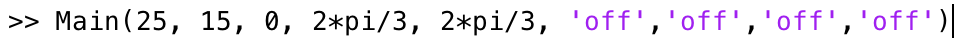
\includegraphics[width=0.75\textwidth]{figures/sample1.png}
\caption{Command for a cell with aspect ratio 25:15, on-center spindle, symmetric MT asters (spread of 2$\pi$/3), no push bands, no anterior-to-posterior asymmetry, no length dependent pulling forces, and no MT elasticity.}
\end{figure}

\begin{figure}[H]
\centering
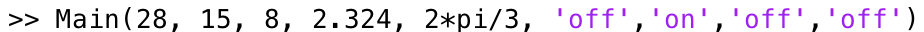
\includegraphics[width=0.75\textwidth]{figures/sample2.png}
\caption{Command for a cell with aspect ratio 28:15, off-center spindle (shifted right by 8 units), asymmetric MT asters ($\phi_1 = 2.324$, $\phi_2 = 2\pi/3$), no push bands, anterior-to-posterior asymmetry, no length dependent pulling forces, and no MT elasticity.}
\end{figure}

\begin{figure}[H]
\centering
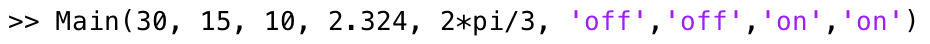
\includegraphics[width=0.75\textwidth]{figures/sample3.png}
\caption{Command for a cell with aspect ratio 30:15, off-center spindle (shifted right by 10 units), asymmetric MT asters ($\phi_1 = 2.324$, $\phi_2 = 2\pi/3$), no push bands, no anterior-to-posterior asymmetry, length dependent pulling forces, and no MT elasticity.}
\end{figure}

\subsection{.mat files}
\noindent\texttt{dyneins16to30.mat}: Contains a cell of vectors, where cell index \texttt{a} corresponds to the vector of dynein locations for given input \texttt{a} to \texttt{Main.m} (\texttt{b} is fixed at 15). \\[3pt]

\noindent\texttt{dyneins\_b16to35.mat}: Contains a cell of vectors, where cell index \texttt{b} corresponds to the vector of dynein locations for given input \texttt{b} to \texttt{Main.m} (\texttt{a} is fixed at 15).\\[3pt]

\noindent\texttt{dyneinsAR1p67VolScaleBy1p6.mat}: Contains two different vectors of dynein locations specific to a cell with \texttt{a = 40} and \texttt{b = 24}. These dimensions give us wild type aspect ratio (AR = 1.67) but with cell volume scaled up (from the usual \texttt{a = 25} and \texttt{b = 15}) by a factor of 1.6. The first vector of dynein positions, \texttt{scaleDynWithVol}, is for when we scale the number of dyneins with total arc length so that the arc length between dyneins remains a constant 1. The second vector of dynein positions, \texttt{fixDynAt128}, is for when we fix the number of dyneins to be 128, which is the same number of dyneins as when \texttt{a = 25} and \texttt{b = 15}. \\[3pt]

\noindent\texttt{kValsCtrlAR1p06to2.mat}: Contains vector \texttt{kvec} of scale factors \texttt{k} for \texttt{PDFplotCTRL.m}.

\section{Fitting the parameter \texttt{k\_1}}
\label{fit}
Earlier work with this model included fitting the unknown parameter \texttt{k\_1}, where
\[
k_1 = \frac{1}{\eta \: D}, \qquad \eta = \text{drag coefficient, and }D = \text{diffusion coefficient.}
\]
This fitting was done using the file \texttt{plotPDF.m}. This function takes as input a vector of final angles \texttt{psi} from the computational model and the maximum value of the energy landscape \texttt{Wmax}. It calls the function \texttt{nhist} (written by Johnathan Lansey, open source) to plot a normalized histogram of final angles. Finally, it fits the steady-state p.d.f,
\[
p(\alpha) = e^{-\texttt{k\_1}W(\alpha)},
\] 
to this histogram using a least-squares method (Matlab's \texttt{lsqcurvefit} function) with respect to the unknown parameter \texttt{k\_1}.
\end{document}
